\documentclass[11pt]{article}

\usepackage[utf8]{inputenc}
\usepackage[T1]{fontenc}
\usepackage[margin=1in]{geometry}
\usepackage{amsmath}
\usepackage{graphicx}
\usepackage{float}
\usepackage{booktabs}
\usepackage{array}
\usepackage{caption}
\usepackage[table]{xcolor}
\usepackage[hidelinks]{hyperref}

\graphicspath{{figures/}}
\captionsetup{font=small,labelfont=bf}
\setlength{\parskip}{0.4em}
\renewcommand{\arraystretch}{1.1}

\title{\textbf{Atomistic Fr\'echet Distance (AFD)}\\[0.3em]
\large Method, Sensitivity Analysis, and Results}
\author{Atomistic Evaluation}
\date{\today}

\begin{document}
\maketitle

\begin{abstract}
\noindent
AFD is a distributional, feature-based score for 3D atomistic generative models --- the
Fr\'echet Inception Distance recipe with the Inception network replaced by a pretrained
chemistry-aware encoder. This report summarizes the method, a validation/sensitivity
study establishing when AFD is statistically valid and how strongly it reacts to
controlled degradations, and current AFD scores for a panel of published molecule
and materials generators alongside preliminary legacy metrics.
\end{abstract}

%======================================================================
\section{AFD: Method}
%======================================================================

AFD (\emph{Atomistic Fr\'echet Distance}) is ``FID for atoms'': the same recipe as the
Fr\'echet Inception Distance used to score image generators, with the Inception-v3 image
encoder replaced by a \textbf{Conditional Equivariant Transformer (CT)} pretrained on
atomistic data. Every structure --- reference and generated --- is embedded through the
frozen CT, harvesting its 256-dimensional graph-level embedding (\texttt{mol\_emb}). A
Gaussian $(\mu,\Sigma)$ is fit to each set of embeddings, and AFD reports the closed-form
Fr\'echet (Wasserstein-2) distance between the two Gaussians:
%
\begin{equation}
\mathrm{AFD}^2 \;=\; \lVert \mu_r - \mu_g \rVert_2^{\,2}
\;+\; \operatorname{Tr}\!\Big( \Sigma_r + \Sigma_g - 2\big(\Sigma_r \Sigma_g\big)^{1/2} \Big),
\end{equation}
%
where $(\mu_r,\Sigma_r)$ and $(\mu_g,\Sigma_g)$ are the reference and generated
embedding statistics. \textbf{Lower is better}; $\mathrm{AFD}=0$ means the generated set
is distributionally indistinguishable from the reference \emph{in the CT feature space}.
The point of this distribution-matching formulation is that AFD is a single,
\emph{set-level} score: it does not require per-sample labels, one-to-one matching, or a
tractable likelihood. It asks only how faithfully the entire generated distribution
reproduces a known ground-truth distribution in a chemistry-aware feature space, capturing
drift in geometry, in composition, or in both at once.

The Fr\'echet form is attractive because it is closed-form and cheap --- it needs only the
first two moments of each feature set and reduces to a matrix square root --- yet it still
registers both a shift in the mean embedding and a change in the covariance (spread) of the
distribution. Its shortcomings follow from the same assumption: modeling each feature set as
a single Gaussian keeps only those first two moments, so AFD is blind to higher-order
distributional structure, and the estimator is \emph{biased upward} with a bias that grows as
$N$ shrinks --- scores at different sample sizes are not comparable, and below the 256-d
feature rank the covariance is degenerate and the number is meaningless (see
Section~\ref{sec:sensitivity}). A second class of limitations comes from building the metric
on \textbf{features from a pretrained model}: the checkpoint is part of the metric, so two AFD
numbers are only comparable if produced with the same checkpoint against the same reference,
and the domain-matched checkpoint must be used (an in-domain encoder is dramatically more
sensitive than a cross-domain one, Section~\ref{sec:checkpoint}). The score also inherits the
encoder's invariances --- the CT embedding is E(3)-invariant and effectively intensive, so AFD
is blind to chirality and to unit-cell multiplicity --- and, being a single distributional
number, it neither localizes which atoms drifted nor certifies that any individual structure
is physically valid. AFD is therefore a comparative, distributional metric to be paired with
validity/stability/novelty checks, not a replacement for them.

%======================================================================
\section{AFD Sensitivity Analysis}
\label{sec:sensitivity}
%======================================================================

A sensitivity analysis establishes \emph{when} AFD is a trustworthy measure and \emph{how}
it responds to known changes. It answers three questions: (i) how many samples are needed
before a score is statistically valid and rankable --- the finite-$N$ validity floor; (ii)
how small a difference is resolvable at a given $N$ --- the sensitivity floor; and (iii) how
monotonically and how strongly the score reacts to controlled perturbations (position noise,
atom mutation, vacancies, bond/lattice scaling), which both validates the metric and lets us
calibrate a raw AFD value into physical units. Every experiment below compares a ground-truth
reference against a controlled degradation of held-out ground-truth folds (fixed permutation,
seed 2026), with the reference subsampled to match the target $N$ on both sides; bands are
95\% CIs over replicate folds and $\rho$ denotes the Spearman rank correlation. Runtimes are
wall-clock on one RTX~A5000.

\subsection{Sample size and the validity floor}

Figures~\ref{fig:ss_qm9} and~\ref{fig:ss_mp20} measure pure finite-$N$ bias: both sides are
\emph{unperturbed} ground truth, so the true distance is zero and any positive AFD is
estimator bias. Panel~(a) plots the AFD of each disjoint fold against its size $N$ (log--log),
with the per-$N$ mean marked and the 256-d feature-dimension line; below that rank the
covariance is singular and the small-$N$ values ($N=10,100$) are artifacts. Panel~(b) zooms
into the full-rank regime ($N\ge 500$) and fits the floor as
$\mathrm{AFD}\approx \text{intercept}+c/N$, showing that once the covariance is well
resolved the bias decays as $1/N$ toward zero. For QM9 the floor is $0.0105$ at $N{=}500$,
$0.0050$ at $N{=}1{,}000$, $5.5\times10^{-4}$ at $N{=}5{,}000$, and $\approx 0$ at
$N{=}10{,}000$; mp20 follows the same law ($0.022$, $0.011$, $0.0015$ at $N{=}500/1{,}000/5{,}000$).
The practical rules: never compare AFD across different $N$; use $N\ge 500$ for any meaningful
score, $N\ge 1{,}000$ to rank models, and $N\ge 5{,}000$ to resolve gaps of $\sim0.001$
between strong models.

\begin{figure}[H]
\centering
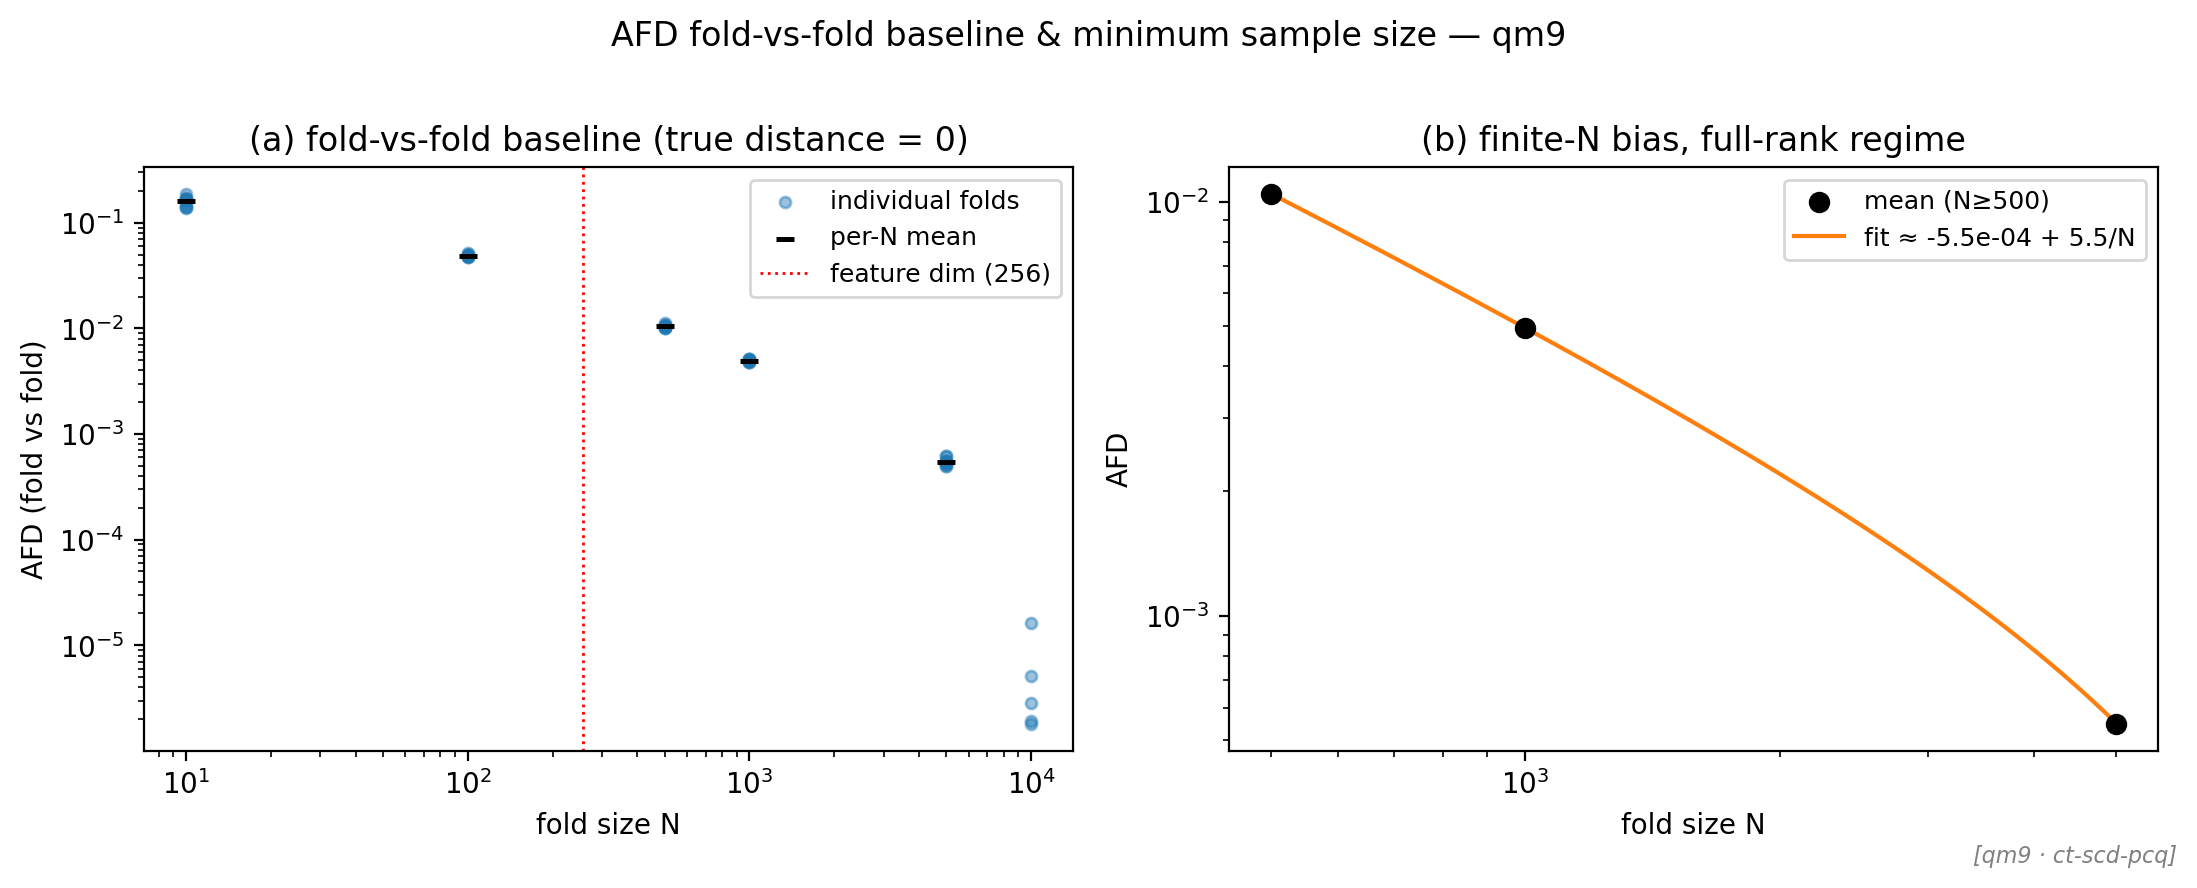
\includegraphics[width=\linewidth]{fig1_sample_size.png}
\caption{QM9 fold-vs-fold baseline (\texttt{ct-scd-pcq}). (a) AFD of individual disjoint
ground-truth folds vs.\ fold size $N$ with per-$N$ means; the covariance is rank-degenerate
left of the 256-d feature line. (b) The full-rank ($N\ge500$) floor decays as $1/N$.
Re-plotted from the raw \texttt{re\_val} results without the mean connecting line, which the
log axis could not draw where the $N{=}10{,}000$ mean reaches the numerical floor.}
\label{fig:ss_qm9}
\end{figure}

\begin{figure}[H]
\centering
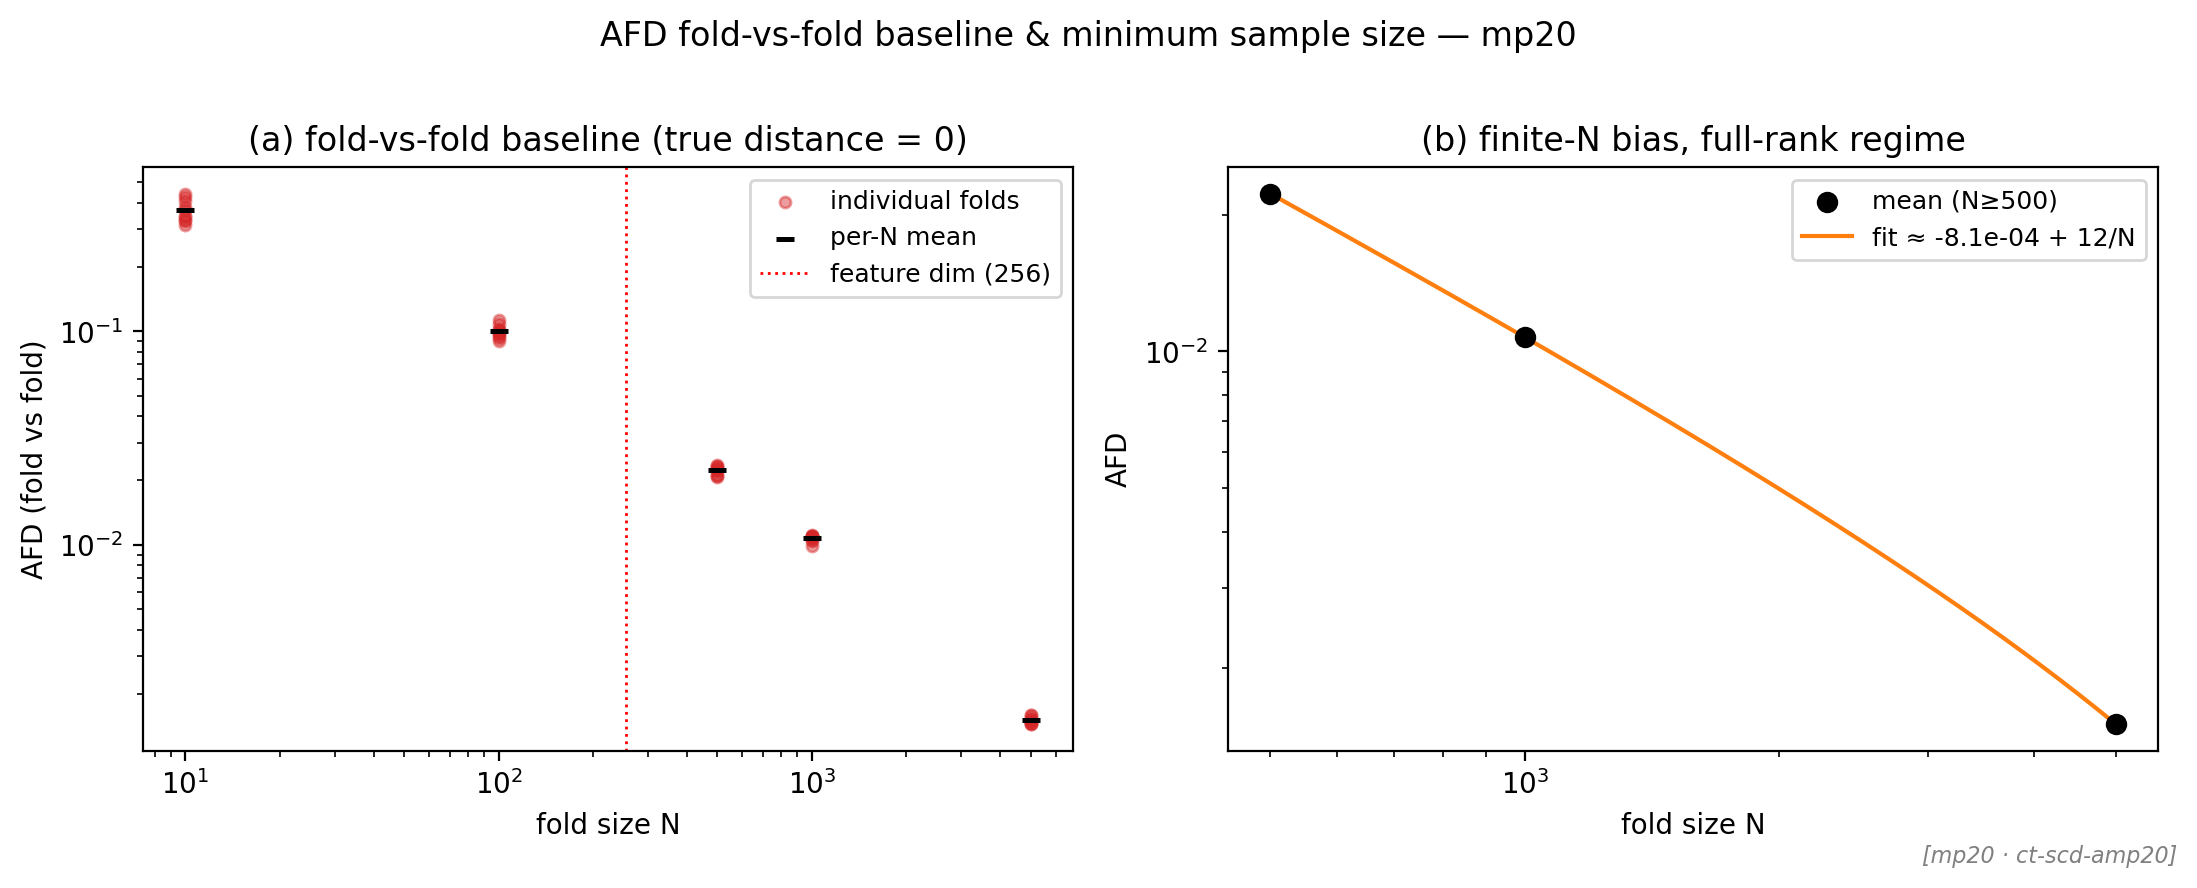
\includegraphics[width=\linewidth]{mp20_fig1_sample_size.png}
\caption{Materials (mp20, \texttt{ct-scd-amp20}) counterpart of Figure~\ref{fig:ss_qm9}: the
same rank floor and $1/N$ finite-$N$ decay.}
\label{fig:ss_mp20}
\end{figure}

\subsection{Molecular sensitivity (QM9)}

The QM9 ladders (Figure~\ref{fig:qm9_ladders}) confirm AFD is monotone and sensitive to
every degradation tested. Position noise sits at the floor for $\sigma\le0.01$~\AA{}, is
resolved by $\sigma\approx0.03$~\AA{} ($0.149$), and saturates near $0.44$ by
$\sigma\approx0.1$~\AA{} ($\rho=0.95$); a \emph{single} mutated atom scores $0.187$ in-set /
$0.289$ for an out-of-distribution (OOD) element, and a single vacancy scores $0.196$
($\rho=1.00$ for mutation and vacancy). Crucially, OOD chemistry (elements absent from the
reference) scores higher than in-set changes at every count. The fine-grid noise sweep
(Figure~\ref{fig:qm9_posnoise}) and the alchemical experiment (Figure~\ref{fig:qm9_alch})
reinforce this: the in-set mutation ladder rises monotonically ($1$ atom $\to0.19$, $5\to0.38$),
and among directed single-atom swaps the OOD C$\to$Si is the largest ($\approx0.37$). Two
useful negative controls appear in Figure~\ref{fig:qm9_bonus}: bond-length scaling is
strongly registered and V-shaped about $1.0$ ($\rho=0.97$), but a molecule and its
\textbf{mirror image} score identically ($0.0060$ vs.\ $0.0061$) --- AFD is blind to
chirality and must be paired with an explicit handedness check.

\begin{figure}[H]
\centering
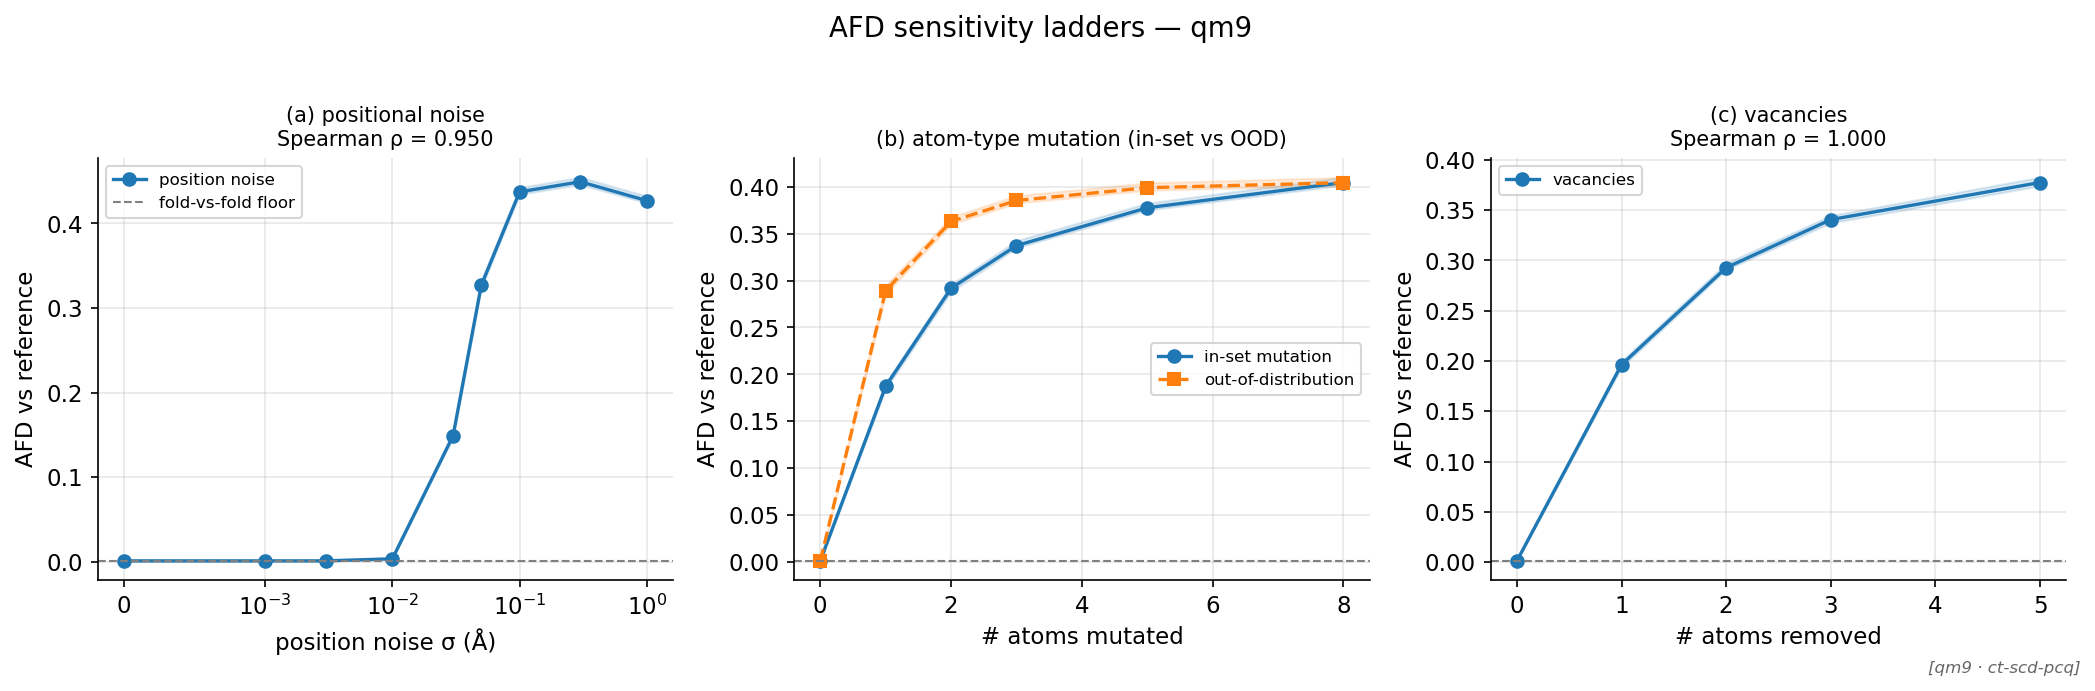
\includegraphics[width=\linewidth]{fig2_ladders.png}
\caption{QM9 sensitivity ladders (mean $+$ 95\% CI vs.\ the fold floor): (a) position noise
$\sigma$; (b) atom-type mutation, in-set (solid) vs.\ OOD (dashed); (c) vacancies. All
monotone; OOD $>$ in-distribution at every count.}
\label{fig:qm9_ladders}
\end{figure}

\begin{figure}[H]
\centering
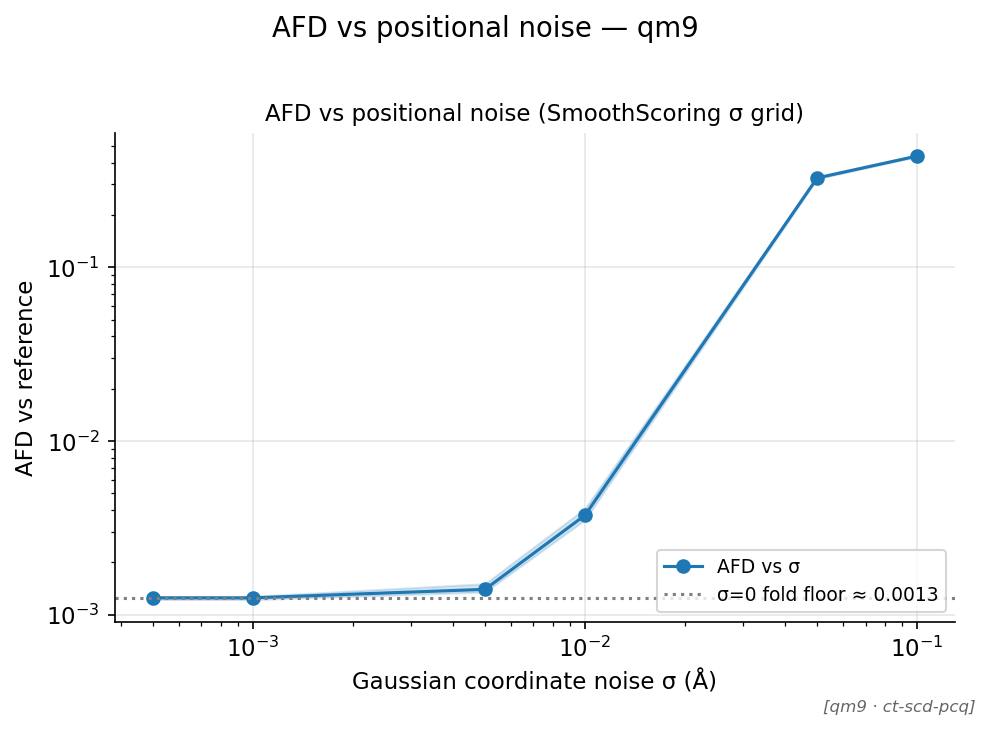
\includegraphics[width=0.82\linewidth]{mv_positional_noise.png}
\caption{QM9 AFD vs.\ Gaussian coordinate noise on a fine $\sigma$ grid (log--log): at the
floor for $\sigma\le0.001$~\AA{}, climbing from $\sigma\approx0.005$--$0.01$~\AA{} to
$\approx0.44$ at $\sigma=0.1$~\AA{}.}
\label{fig:qm9_posnoise}
\end{figure}

\begin{figure}[H]
\centering
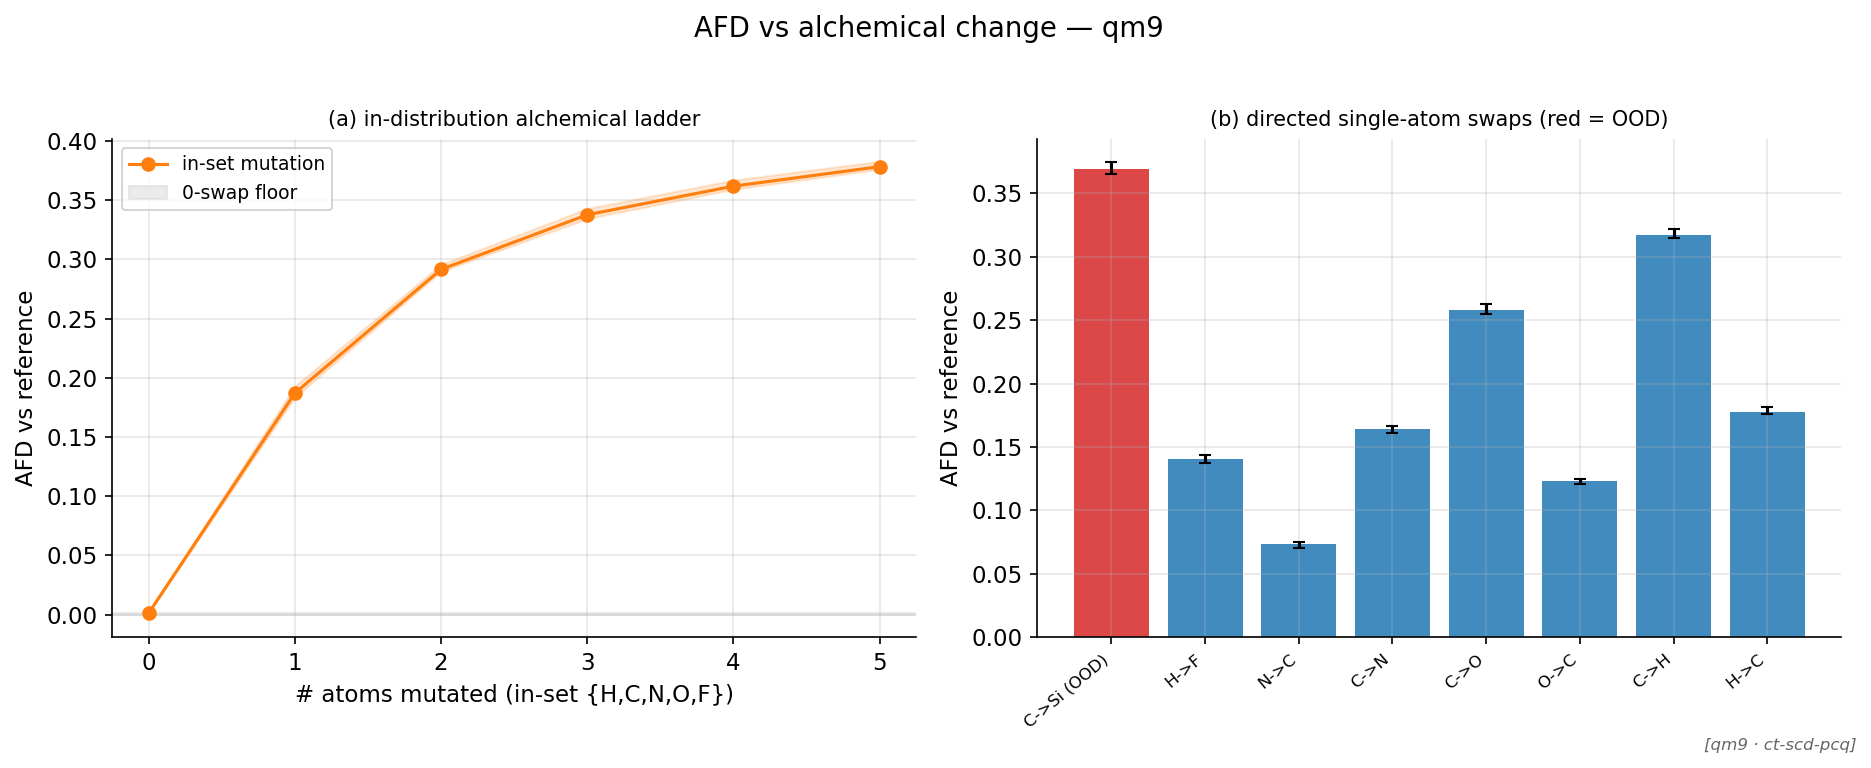
\includegraphics[width=\linewidth]{mv_alchemical.png}
\caption{QM9 alchemical change: (a) integer in-set mutation ladder; (b) directed single-atom
swaps along fixed element directions. The OOD C$\to$Si swap (red) is the largest response.}
\label{fig:qm9_alch}
\end{figure}

\begin{figure}[H]
\centering
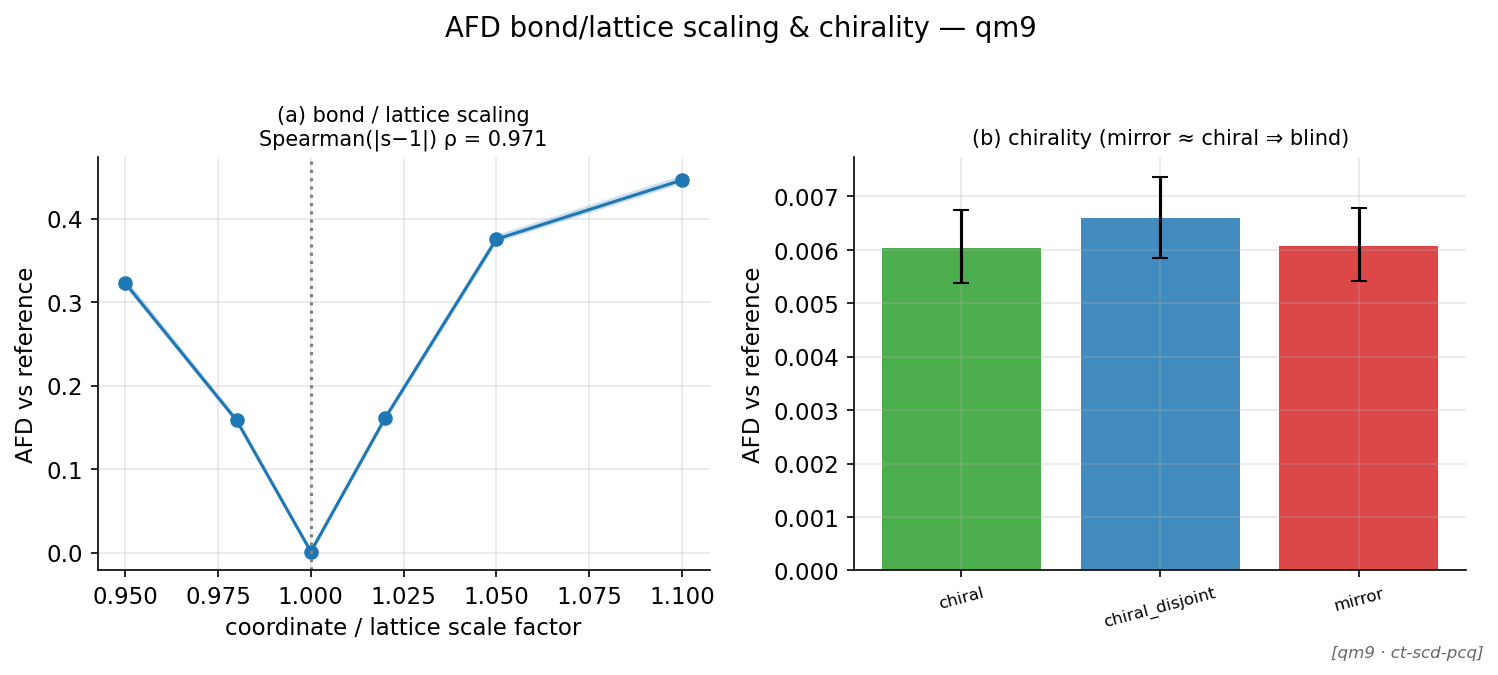
\includegraphics[width=\linewidth]{fig3_bonus.png}
\caption{QM9 bonus tests: (a) AFD vs.\ uniform coordinate scale (V-shaped about $1.0$); (b)
chirality --- a chiral fold, a disjoint chiral fold, and the mirror image of the first all
score alike, confirming AFD is reflection-invariant.}
\label{fig:qm9_bonus}
\end{figure}

\subsection{Materials sensitivity (mp20)}

Periodic crystals behave the same way once positions are wrapped into the (non-orthographic)
unit cell (Figure~\ref{fig:mp20_ladders}): AFD is strongly sensitive and monotone
($\rho=1.00$), detecting $\sigma\approx0.01$~\AA{} ($0.022$) and rising to $0.77$ at
$\sigma=0.1$~\AA{}; one mutated atom scores $0.22$ and one vacancy $0.17$, with transuranic
OOD substitutions again above in-set ($0.85$ vs.\ $0.63$ at 5 atoms). Isotropic lattice
strain is registered as expected (Figure~\ref{fig:mp20_strain}a), but \textbf{unit-cell
repetition} exposes an invariance (Figure~\ref{fig:mp20_strain}b): tiling a crystal into an
$8\times$ supercell leaves AFD near the floor ($0.0049\to0.0070$), because the pooled
embedding is effectively intensive. AFD correctly ignores supercell convention but cannot
flag a wrong cell multiplicity.

\begin{figure}[H]
\centering
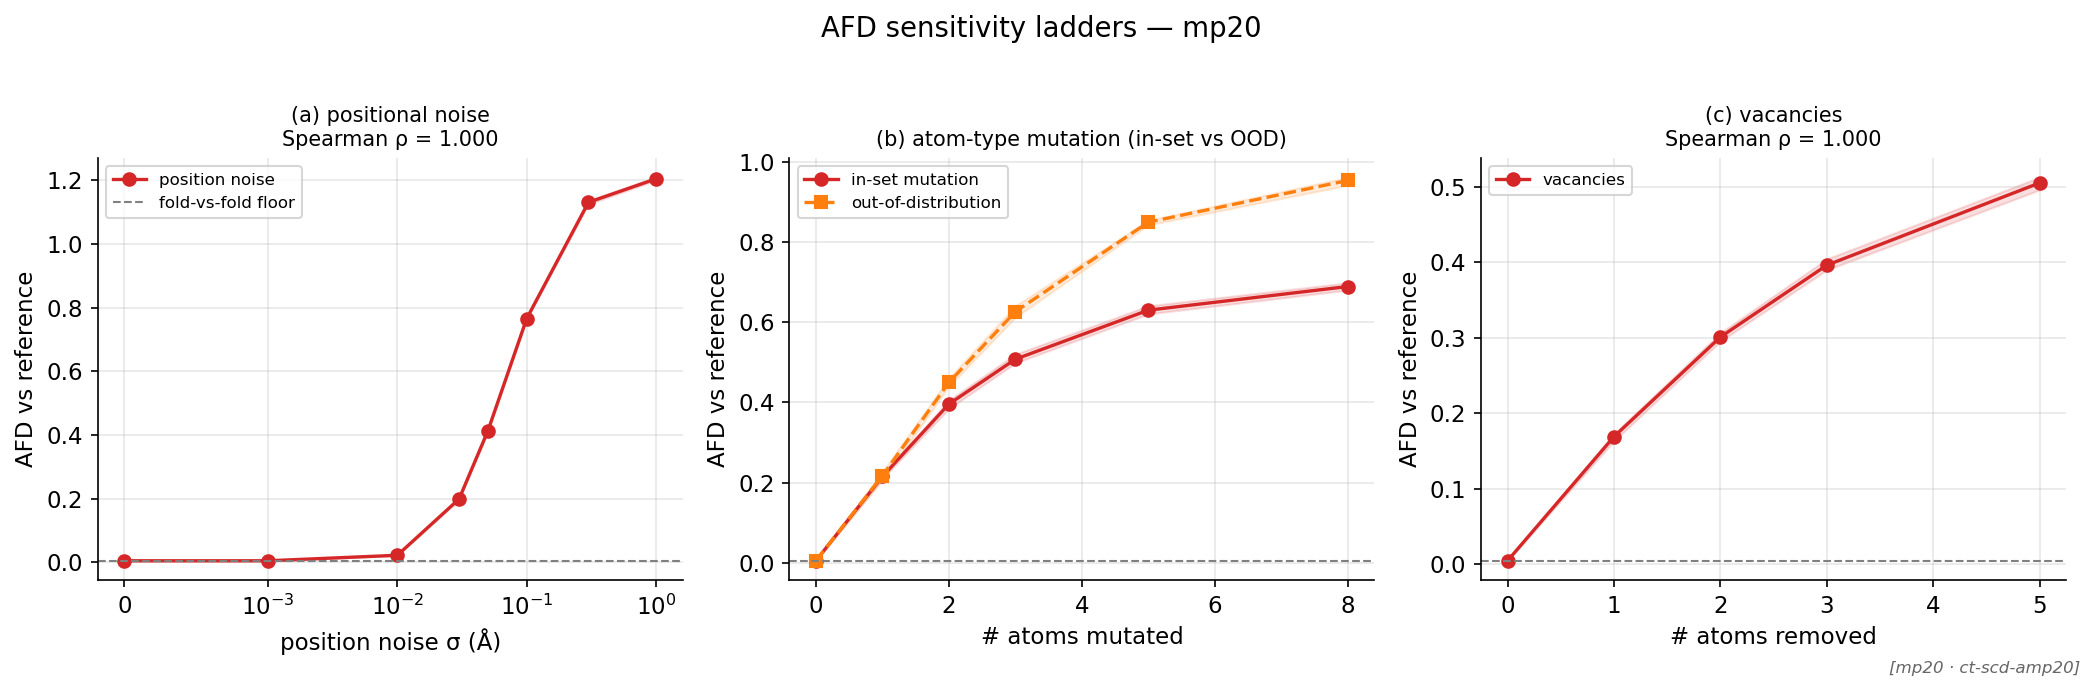
\includegraphics[width=\linewidth]{mp20_fig2_ladders.png}
\caption{mp20 sensitivity ladders: wrapped position noise, atom mutation (in-set vs.\
transuranic OOD), and vacancies vs.\ the fold floor. Comparable sensitivity to QM9 under the
matched checkpoint.}
\label{fig:mp20_ladders}
\end{figure}

\begin{figure}[H]
\centering
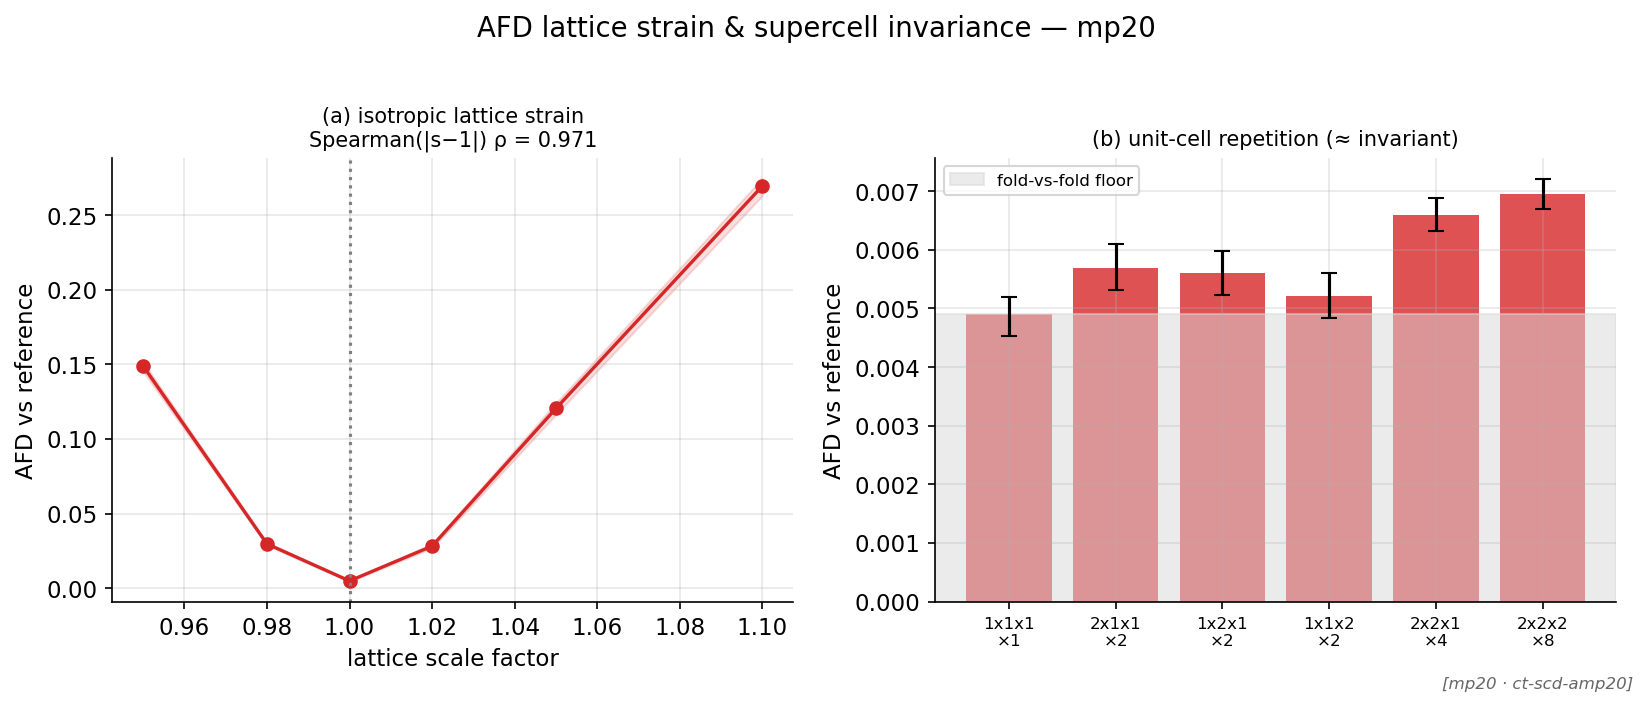
\includegraphics[width=\linewidth]{mp20_fig3_strain_supercell.png}
\caption{mp20 (a) isotropic lattice strain (V-shaped about $1.0$) and (b) unit-cell
repetition $\times1$--$\times8$: AFD stays near the floor under supercell tiling --- an
invariance of the intensive embedding.}
\label{fig:mp20_strain}
\end{figure}

\subsection{Calibration: reading a raw AFD value}

Inverting the monotone QM9 ladders converts a raw AFD number into an equivalent physical
degradation of ground truth (Table~\ref{tab:calibration}). As a rule of thumb, an
\textbf{AFD of $0.1$ corresponds to about $0.023$~\AA{} of coordinate jitter, or roughly half
an atom per molecule mutated or missing}; a single mutated atom registers $\approx0.19$
(in-set) / $\approx0.29$ (OOD), a single vacancy $\approx0.20$.

\begin{table}[H]
\centering
\small
\caption{AFD value $\to$ equivalent QM9 perturbation, by interpolation on the sensitivity
ladders. A ground-truth interpretation aid, not generator scores.}
\label{tab:calibration}
\begin{tabular}{c c c c}
\toprule
AFD level & jitter $\sigma$ (\AA{}) & \# atoms mutated & \# atoms removed \\
\midrule
0.01 & 0.011 & 0.05 & 0.05 \\
0.05 & 0.016 & 0.26 & 0.25 \\
0.10 & 0.023 & 0.53 & 0.51 \\
0.20 & 0.036 & 1.12 & 1.04 \\
0.30 & 0.047 & 2.18 & 2.15 \\
\bottomrule
\end{tabular}
\end{table}

\subsection{Checkpoint dependence}
\label{sec:checkpoint}

Because the feature extractor is a pretrained CT, the checkpoint is part of the metric.
Figures~\ref{fig:cross} and~\ref{fig:ckpt} rerun the position and mutation ladders across
checkpoints. The in-domain specialist dominates every cross-domain alternative: at
$\sigma\approx0.1$~\AA{}, QM9 scores $0.44$ under \texttt{pcq} but only $0.15$ under the
materials checkpoint, and mp20 scores $0.76$ under \texttt{amp20} but $0.004$ under \texttt{pcq}.
Across all four checkpoints (Figure~\ref{fig:ckpt}) the ordering is unambiguous --- the
matched specialist $\gg$ the generalist \texttt{all} $>$ \texttt{omol25} --- so AFD must
always be run with the domain-matched checkpoint.

\begin{figure}[H]
\centering
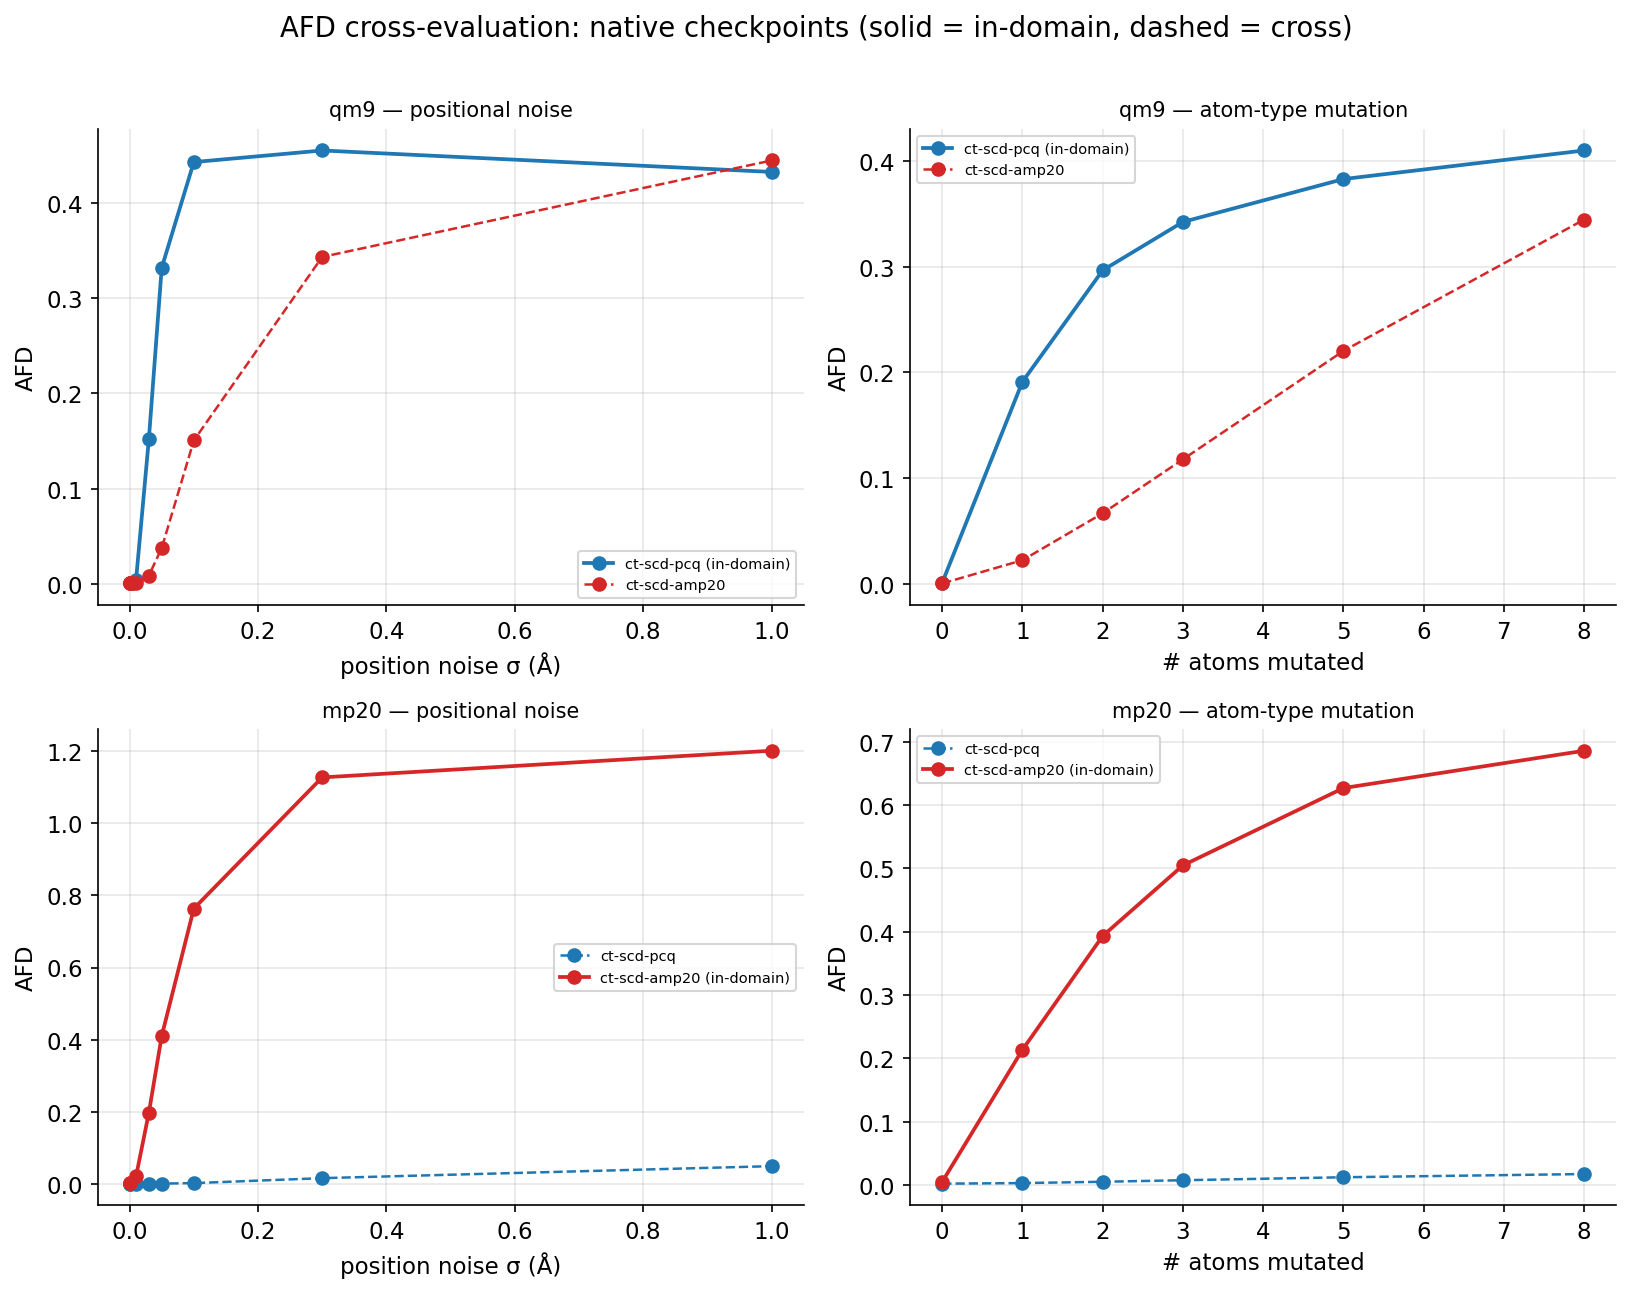
\includegraphics[width=\linewidth]{cross_overlays.png}
\caption{In-domain checkpoint (solid) vs.\ the other native checkpoint (dashed) for each
dataset $\times$ \{position, mutation\}. The in-domain curve dominates everywhere.}
\label{fig:cross}
\end{figure}

\begin{figure}[H]
\centering
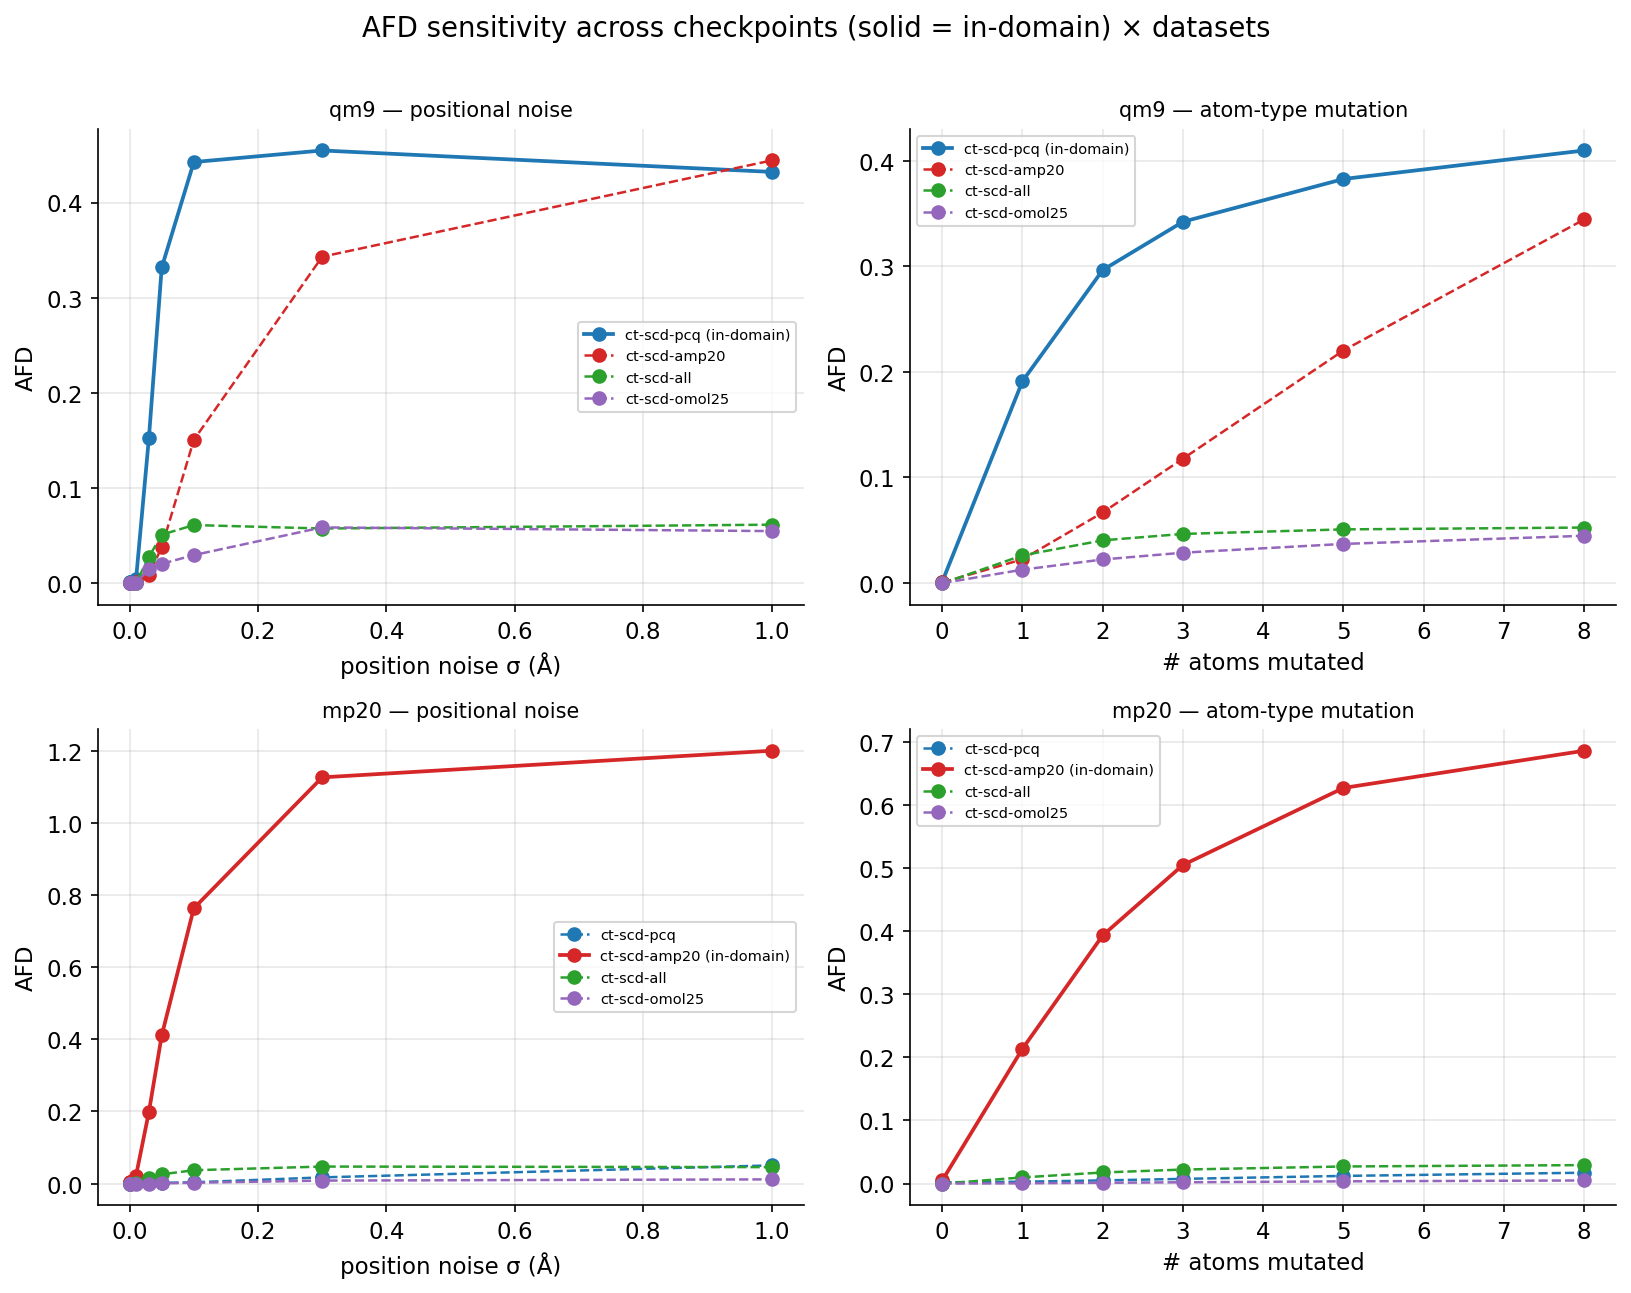
\includegraphics[width=\linewidth]{checkpoint_overlays.png}
\caption{All four checkpoints on the same $2\times2$ grid. The domain-matched specialist is
far more sensitive; the generalist \texttt{all} is a weak runner-up and \texttt{omol25} is
weak on both modalities.}
\label{fig:ckpt}
\end{figure}

\subsection{Application: scoring relaxed geometries}

As a downstream check, AFD reads systematic geometry error and ranks post-processing steps
(Figure~\ref{fig:relaxed}). RDKit force-field conformers of \emph{chemically correct}
molecules already sit far above the floor ($\approx0.19$) purely from geometry. Relaxing them
orders the relaxers correctly: GFN2-xTB pulls the distribution \emph{toward} the DFT reference
($\approx0.106$), while the cheaper GFN-FF pushes it \emph{further away} ($\approx0.242$).
AFD registers both the improvement and the regression.

\begin{figure}[H]
\centering
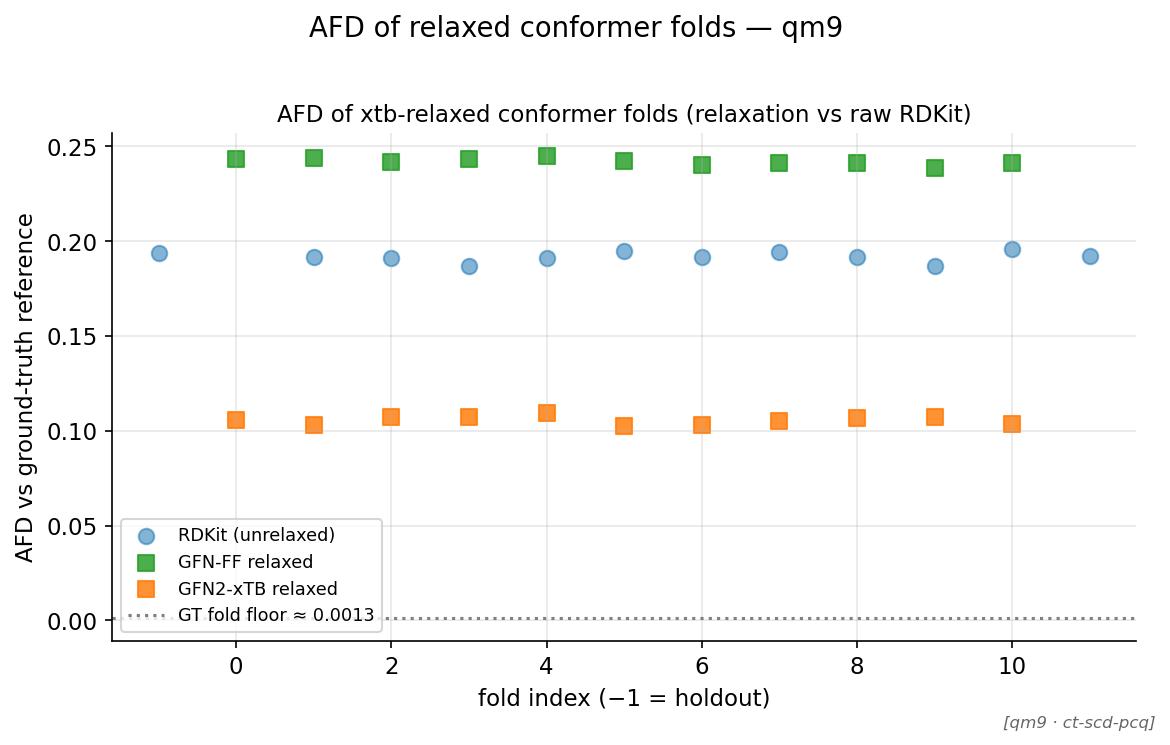
\includegraphics[width=0.82\linewidth]{mv_relaxed_folds.png}
\caption{AFD of RDKit conformers relaxed with GFN-FF and GFN2-xTB vs.\ the DFT-geometry QM9
reference, against raw RDKit and the floor. GFN2-xTB improves on RDKit; GFN-FF regresses.}
\label{fig:relaxed}
\end{figure}

%======================================================================
\section{AFD Results}
%======================================================================

\subsection{AFD scores for existing generative models}

Figures~\ref{fig:afd_qm9}--\ref{fig:afd_geom} plot AFD against average sampling cost for a
panel of published generators on each dataset (log--log; lower AFD is better, and points
toward the lower-left are both faster and more faithful). Models with no timing metadata are
drawn as labeled dashed reference lines. On QM9 (Figure~\ref{fig:afd_qm9}) the strongest
distributional fidelity comes from GCDM and the larger Zatom-J variants
($\mathrm{AFD}\approx0.015$--$0.05$), while ADiT and EDM trail near $0.22$--$0.36$; several
fast samplers (e.g.\ the \texttt{tabasco} and small Zatom models) occupy the low-cost region
at moderate AFD. On mp20 (Figure~\ref{fig:afd_mp20}) the MatterGen variants achieve the
lowest AFD ($0.023$--$0.05$) at high per-sample cost, whereas the invalid-cell--prone
\texttt{Compositional} baseline sits worst ($\approx1.19$); the Zatom and DiffCSP families
span the middle. On GEOM-drugs (Figure~\ref{fig:afd_geom}) \texttt{zatom80M-Jgeom} gives the
best AFD ($0.22$) at by far the lowest cost, with EQGAT next and GeoLDM/ADiT-author highest.
The exact values and timings are collected in
Tables~\ref{tab:eval_qm9}--\ref{tab:eval_geom}.

\begin{figure}[H]
\centering
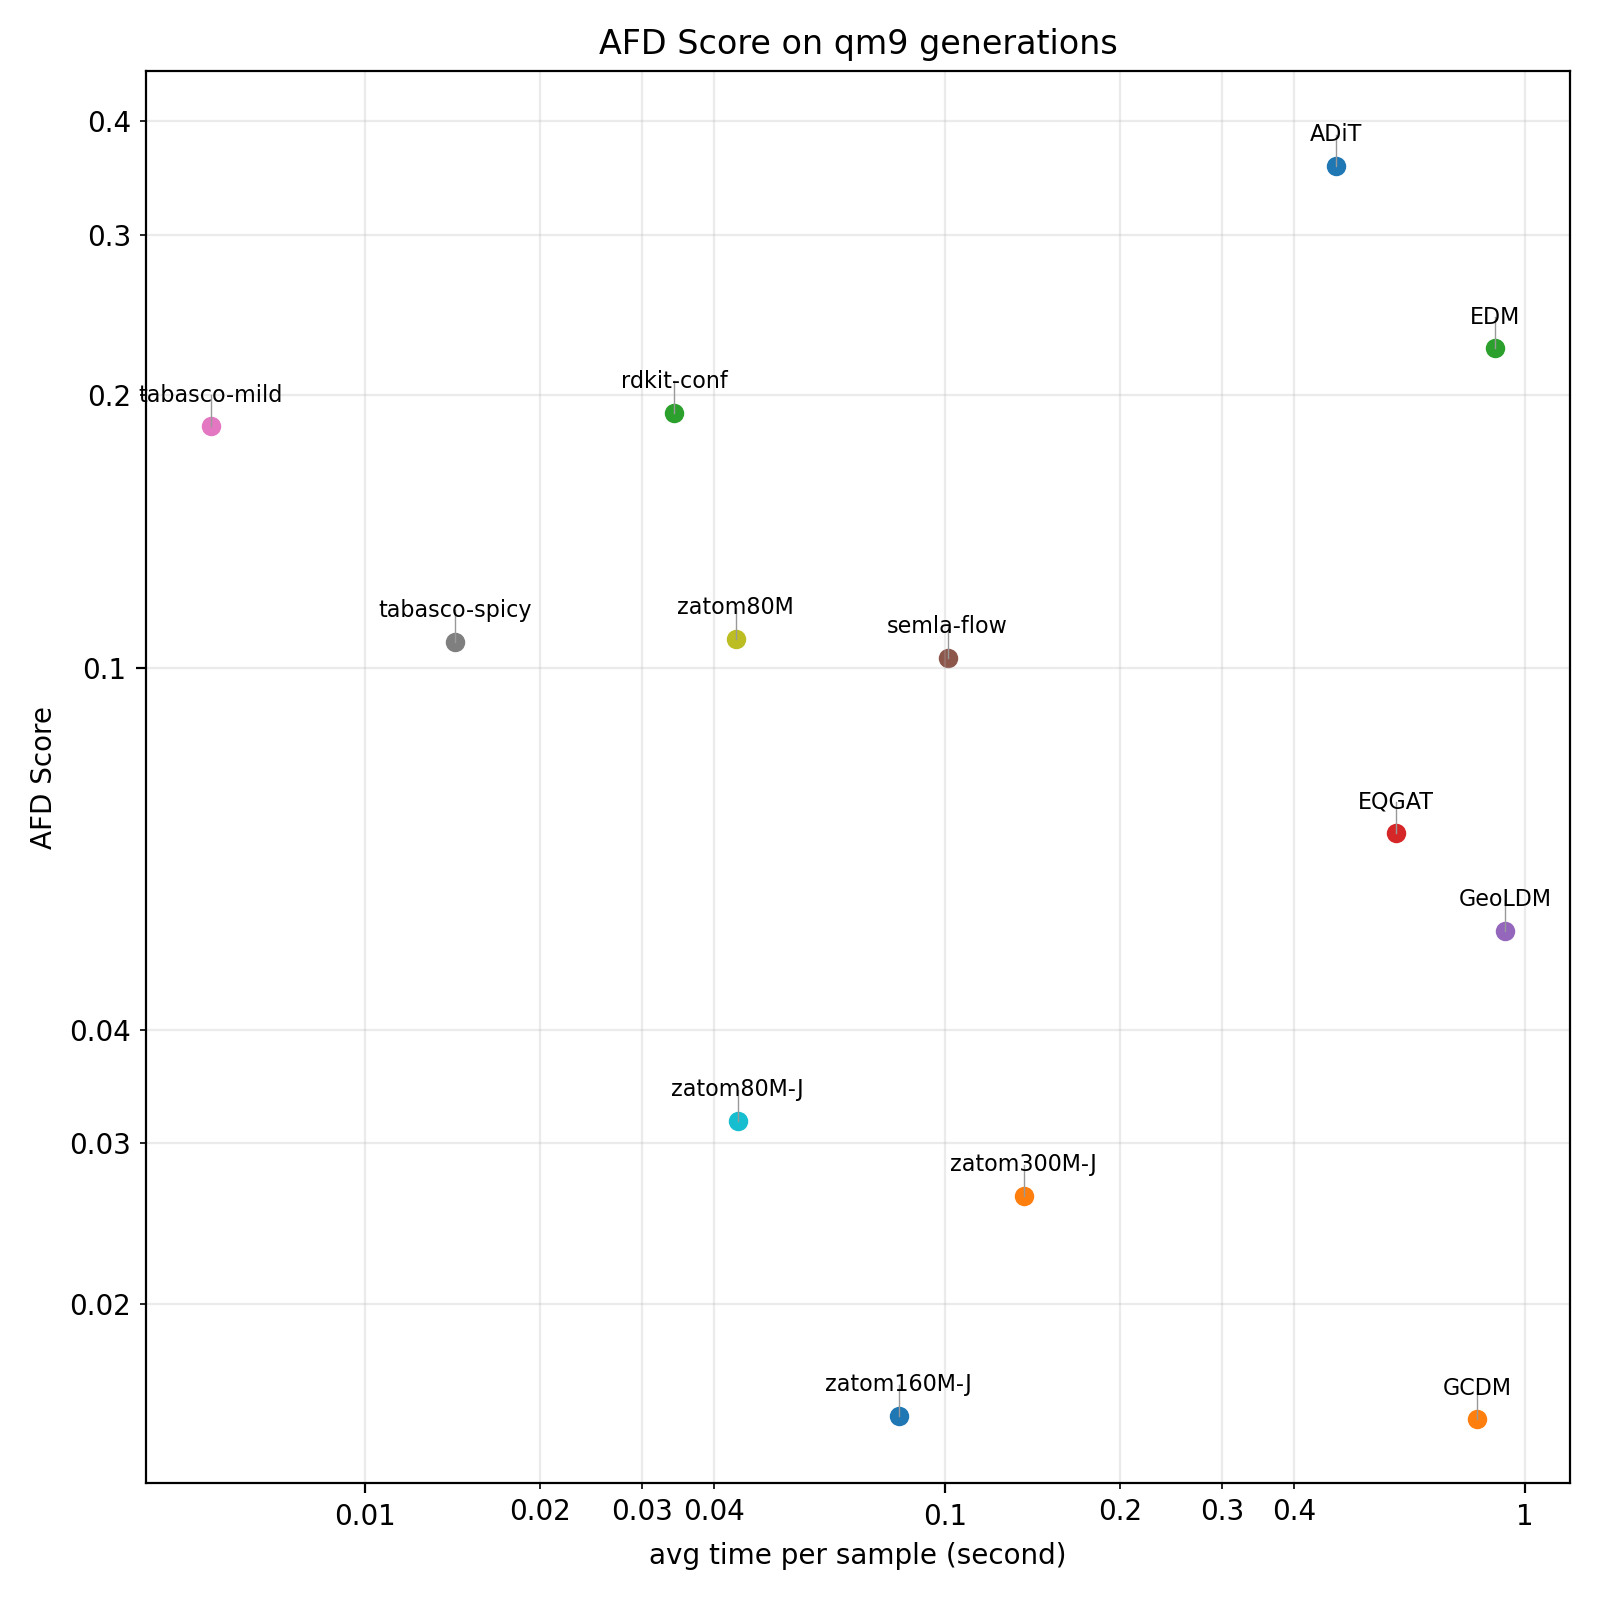
\includegraphics[width=0.72\linewidth]{afd_qm9.png}
\caption{AFD vs.\ average time per sample on QM9 generations.}
\label{fig:afd_qm9}
\end{figure}

\begin{figure}[H]
\centering
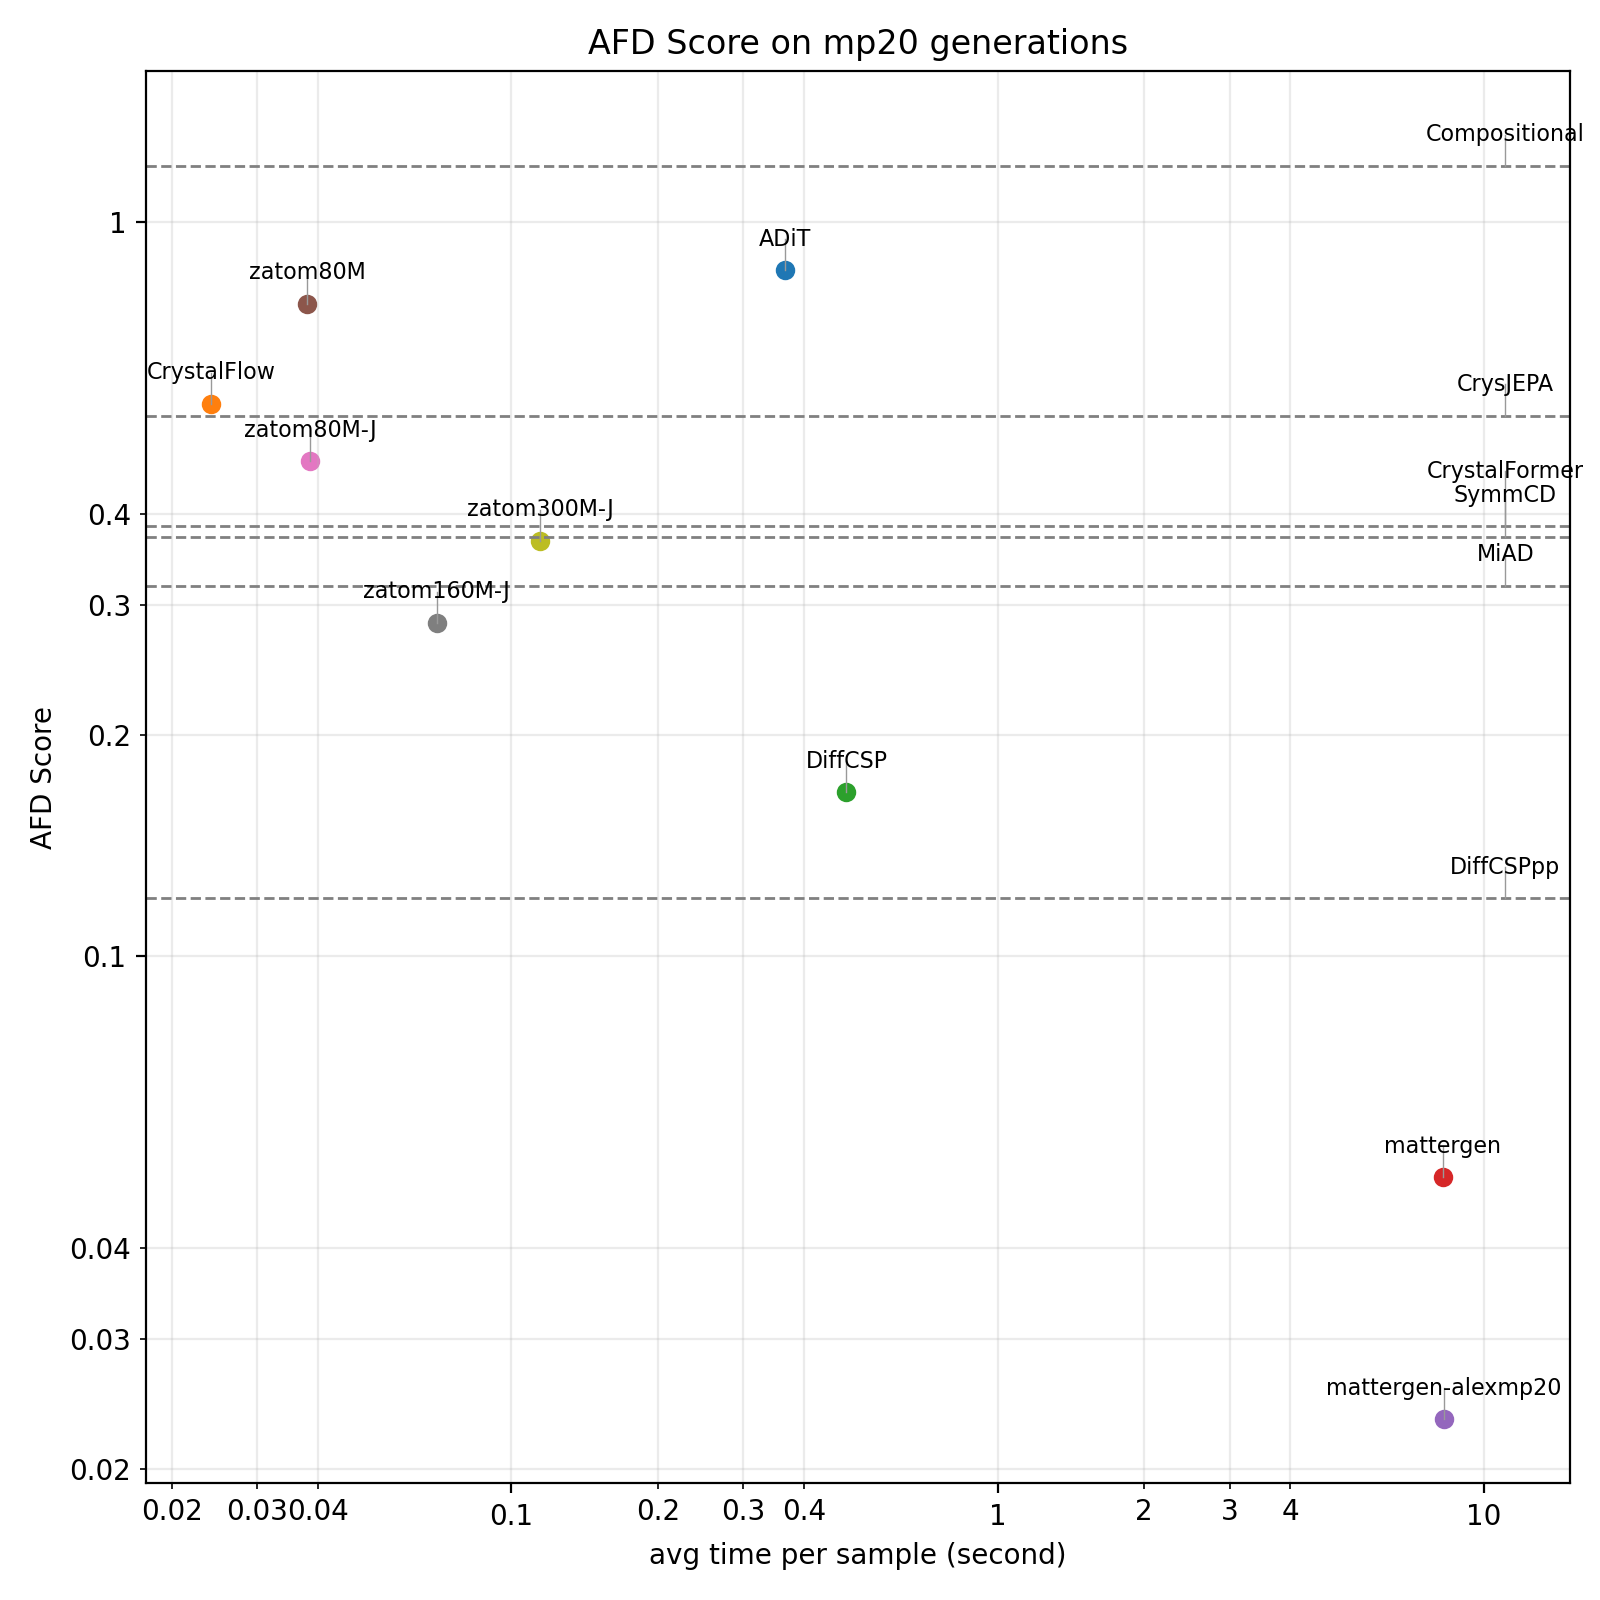
\includegraphics[width=0.72\linewidth]{afd_mp20.png}
\caption{AFD vs.\ average time per sample on mp20 generations (the \texttt{mp20} and
\texttt{mp20\_alt} model sets merged).}
\label{fig:afd_mp20}
\end{figure}

\begin{figure}[H]
\centering
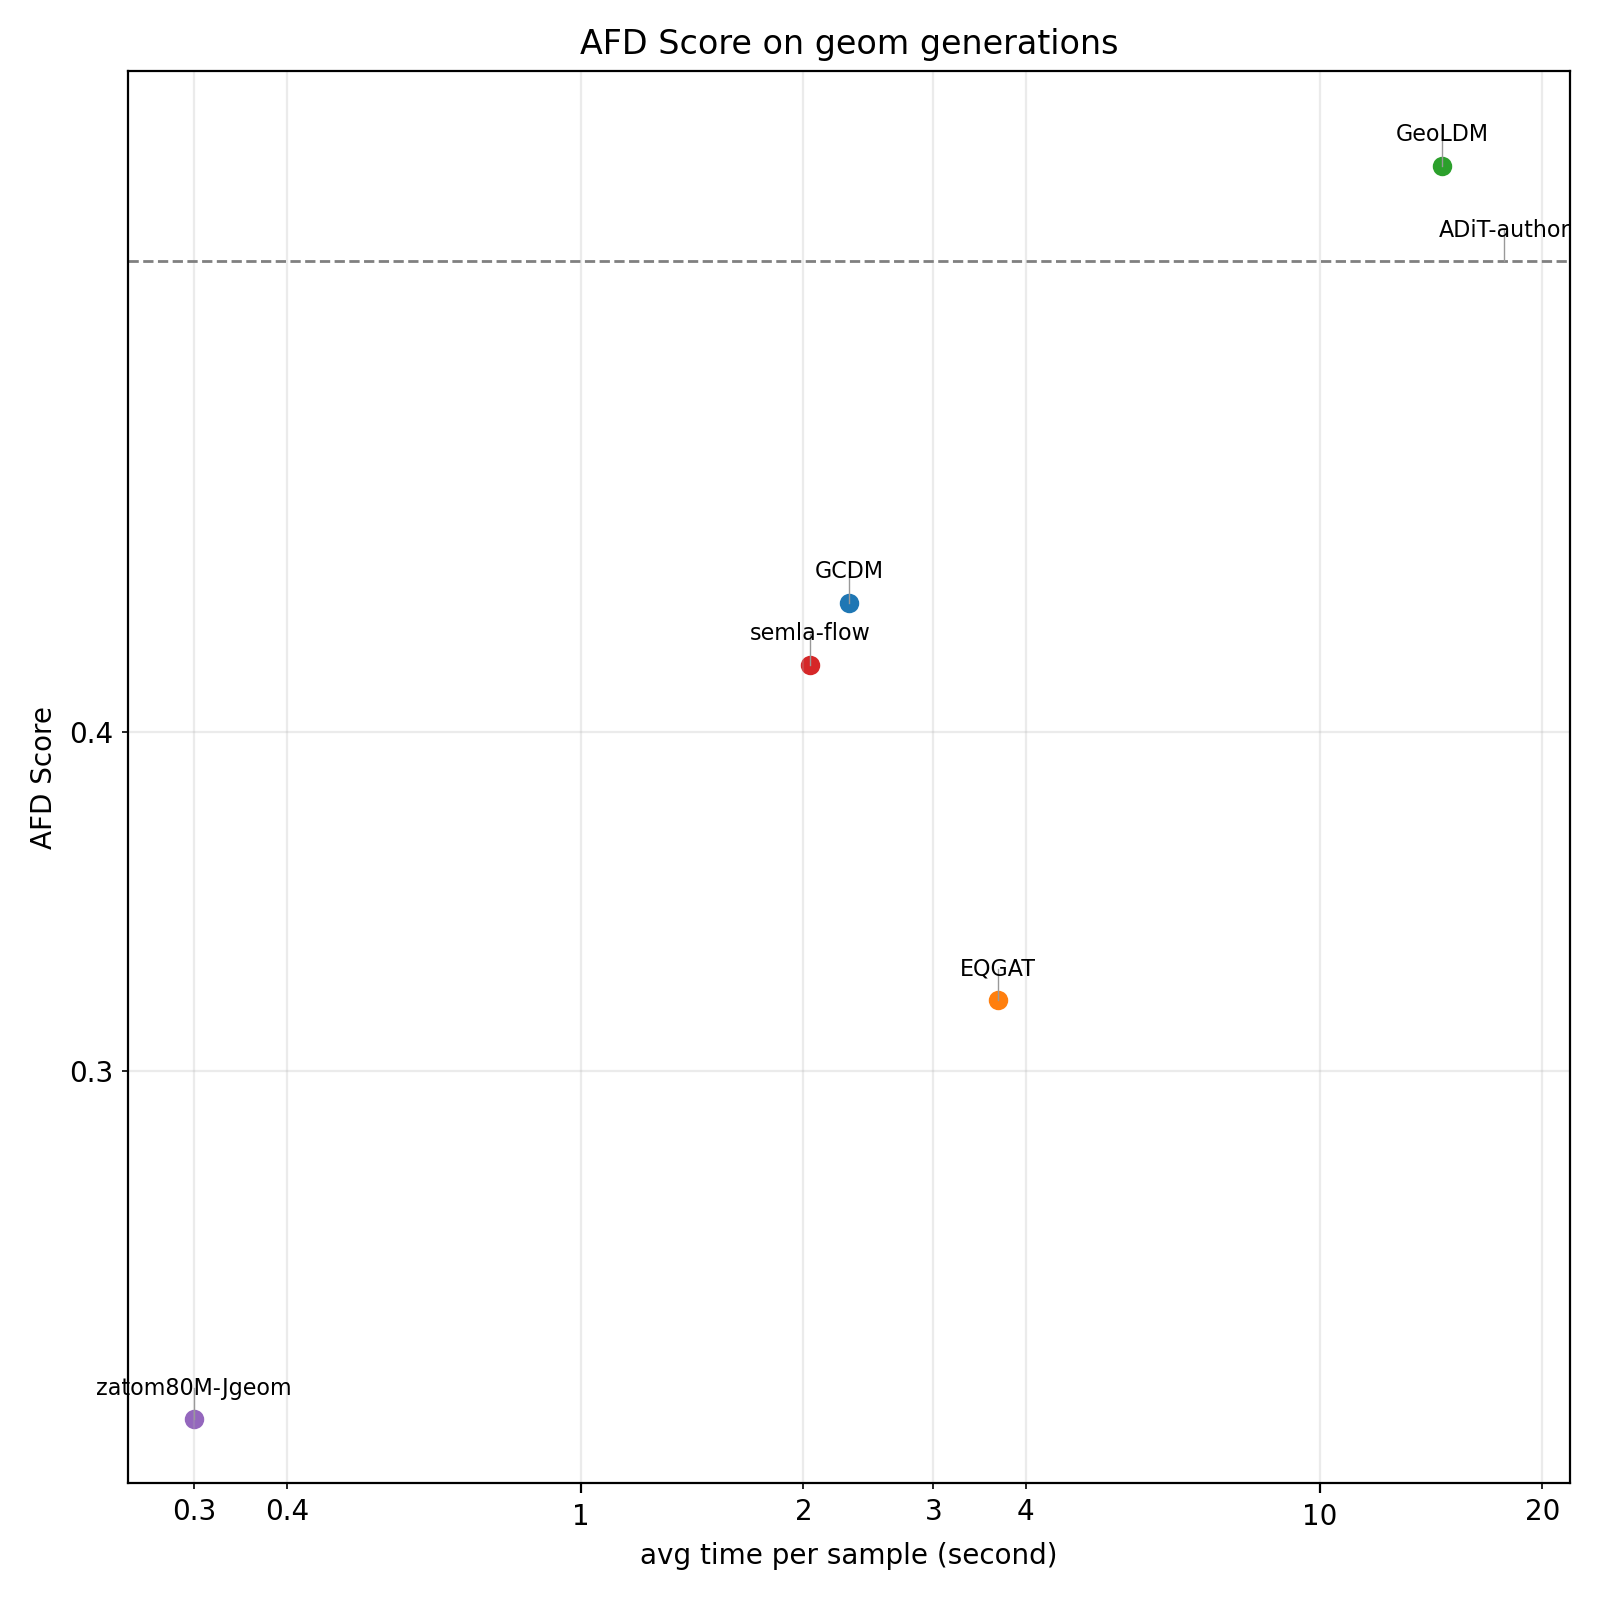
\includegraphics[width=0.72\linewidth]{afd_geom.png}
\caption{AFD vs.\ average time per sample on GEOM-drugs generations.}
\label{fig:afd_geom}
\end{figure}

Tables~\ref{tab:eval_qm9}--\ref{tab:eval_geom} report, per generation set, the AFD score and
the average time per sample. Lower is better in every column; the \textbf{best} value per
column is bold and the \underline{second best} underlined, and rows are ordered by AFD score
from highest (worst) at the top to lowest (best) at the bottom.

\begin{table}[H]
\centering
\small
\caption{QM9 generation scores. Lower is better; \textbf{best} / \underline{second best} per
column.}
\label{tab:eval_qm9}
\begin{tabular}{l r r}
\toprule
Model & AFD score & time/sample (s) \\
\midrule
ADiT          & 0.3569 & 0.4709 \\
EDM           & 0.2249 & 0.8875 \\
rdkit-conf    & 0.1911 & 0.03408 \\
tabasco-mild  & 0.1845 & \textbf{0.005421} \\
zatom80M      & 0.1078 & 0.04352 \\
tabasco-spicy & 0.1070 & \underline{0.01428} \\
semla-flow    & 0.1027 & 0.101 \\
EQGAT         & 0.0659 & 0.5992 \\
GeoLDM        & 0.0514 & 0.9238 \\
zatom80M-J    & 0.0318 & 0.04389 \\
zatom300M-J   & 0.0263 & 0.1365 \\
zatom160M-J   & \underline{0.0150} & 0.08316 \\
GCDM          & \textbf{0.0149} & 0.8257 \\
\bottomrule
\end{tabular}
\end{table}

\begin{table}[H]
\centering
\small
\caption{mp20 generation scores (\texttt{mp20} and \texttt{mp20\_alt} merged). Lower is
better; \textbf{best} / \underline{second best} per column.}
\label{tab:eval_mp20}
\begin{tabular}{l r r}
\toprule
Model & AFD score & time/sample (s) \\
\midrule
Compositional      & 1.1899 & --- \\
ADiT               & 0.8578 & 0.3655 \\
zatom80M           & 0.7732 & \underline{0.03798} \\
CrystalFlow        & 0.5643 & \textbf{0.02408} \\
CrysJEPA           & 0.5440 & --- \\
zatom80M-J         & 0.4714 & 0.0385 \\
CrystalFormer      & 0.3852 & --- \\
SymmCD             & 0.3722 & --- \\
zatom300M-J        & 0.3670 & 0.1147 \\
MiAD               & 0.3189 & --- \\
zatom160M-J        & 0.2838 & 0.07021 \\
DiffCSP            & 0.1669 & 0.4885 \\
DiffCSPpp          & 0.1197 & --- \\
mattergen          & \underline{0.0499} & 8.227 \\
mattergen-alexmp20 & \textbf{0.0234} & 8.267 \\
\bottomrule
\end{tabular}
\end{table}

\begin{table}[H]
\centering
\small
\caption{GEOM-drugs generation scores. Lower is better; \textbf{best} / \underline{second
best} per column.}
\label{tab:eval_geom}
\begin{tabular}{l r r}
\toprule
Model & AFD score & time/sample (s) \\
\midrule
GeoLDM         & 0.6456 & 14.63 \\
ADiT-author    & 0.5955 & --- \\
GCDM           & 0.4460 & 2.304 \\
semla-flow     & 0.4232 & \underline{2.044} \\
EQGAT          & \underline{0.3187} & 3.669 \\
zatom80M-Jgeom & \textbf{0.2235} & \textbf{0.2994} \\
\bottomrule
\end{tabular}
\end{table}

\subsection{Legacy evaluations}

The tables below report a separate, established evaluation suite (validity, uniqueness,
novelty, Fr\'echet ChemNet Distance for molecules, and MLIP-based stability/energy/SUN for
materials). \textbf{These results are preliminary and subject to change.} Rows are ordered
worst (top) to best (bottom) by a composite mean-rank across the direction-corrected metrics;
\textbf{best} / \underline{second best} per column are highlighted among generated models, and
ground-truth (GT) rows are shown for reference but excluded from highlighting. Per-molecule
PoseBusters geometry checks are near-identical to the \texttt{valid} fraction and are omitted
for brevity.

On QM9 (Table~\ref{tab:legacy_qm9}) the RDKit-conformer control is essentially GT-level, and
among true generators the Zatom-J models and EDM lead the composite; EDM pays for its high
novelty with the lowest validity, illustrating the validity/novelty trade-off.

\begin{table}[H]
\centering
\small
\caption{Legacy QM9 molecule metrics (full $\sim$10k sets, GT matched at 10k). FCD lower is
better; others higher is better.}
\label{tab:legacy_qm9}
\begin{tabular}{l r r r r r}
\toprule
Model & rank & valid & novel & unique & FCD \\
\midrule
EDM           & 11.73 & 0.766 & \textbf{0.606} & \underline{0.990} & 0.648 \\
tabasco-spicy & 11.73 & 0.829 & 0.190 & 0.958 & 0.432 \\
tabasco-mild  & 11.45 & 0.814 & 0.281 & 0.973 & 0.372 \\
semla-flow    & 9.91  & 0.899 & 0.187 & 0.840 & 1.085 \\
zatom80M      & 9.64  & 0.860 & 0.192 & 0.971 & \underline{0.098} \\
GCDM          & 8.82  & 0.871 & \underline{0.463} & 0.981 & 0.426 \\
GeoLDM        & 7.36  & 0.907 & 0.420 & 0.979 & 0.192 \\
EQGAT         & 6.64  & 0.910 & 0.410 & 0.977 & 0.164 \\
zatom300M-J   & 6.64  & 0.919 & 0.135 & 0.964 & 0.122 \\
ADiT          & 6.09  & 0.921 & 0.239 & 0.966 & 0.177 \\
zatom80M-J    & 5.36  & 0.922 & 0.150 & 0.963 & 0.112 \\
zatom160M-J   & 4.45  & \underline{0.936} & 0.109 & 0.968 & 0.105 \\
rdkit-conf    & 2.27  & \textbf{0.954} & 0.001 & \textbf{1.000} & \textbf{0.048} \\
\midrule
qm9\_GT (GT)  & 1.90  & 0.946 & 0.002 & 1.000 & 0.050 \\
\bottomrule
\end{tabular}
\end{table}

On mp20 (Table~\ref{tab:legacy_mp20}) the picture is more mixed: MatterGen and MiAD lead the
composite on validity and hull energy, while the Zatom-J models top the (meta)stability and
SUN/MSUN columns; the \texttt{Compositional} baseline is near-perfect on composition validity
but fails structural validity and hull energy.

\begin{table}[H]
\centering
\scriptsize
\setlength{\tabcolsep}{4pt}
\caption{Legacy mp20 materials metrics (full $\sim$10k lightweight; MLIP stability/SUN on
2{,}000 samples). \texttt{e\_hull} lower is better; others higher is better.}
\label{tab:legacy_mp20}
\begin{tabular}{l r r r r r r r r r}
\toprule
Model & rank & valid & unique & nov & stable & metastab. & e\_hull & sun & msun \\
\midrule
SymmCD             & 12.27 & 0.735 & 0.987 & 0.964 & 0.021 & 0.116 & 3.580 & 0.019 & 0.081 \\
Compositional      & 11.91 & 0.220 & 0.953 & 1.000 & 0.004 & 0.004 & 12.522 & 0.004 & 0.001 \\
CrystalFormer      & 11.27 & 0.699 & 0.996 & 0.981 & 0.021 & 0.160 & 7.697 & 0.020 & 0.117 \\
CrystalFlow        & 10.09 & 0.872 & 0.990 & \textbf{1.000} & 0.018 & 0.038 & 1.141 & 0.018 & 0.019 \\
CrysJEPA           & 9.82  & \textbf{0.964} & 0.449 & \underline{1.000} & 0.018 & 0.041 & 0.649 & 0.011 & 0.015 \\
zatom80M           & 9.82  & 0.725 & 0.933 & 0.998 & 0.018 & 0.161 & 2.681 & 0.018 & 0.139 \\
DiffCSPpp          & 9.18  & 0.948 & 0.994 & 0.987 & 0.024 & 0.144 & 0.610 & 0.024 & 0.111 \\
ADiT               & 8.82  & 0.906 & 0.963 & 0.999 & 0.028 & 0.066 & 0.853 & 0.028 & 0.035 \\
zatom80M-J         & 8.00  & 0.885 & 0.901 & 0.993 & \underline{0.034} & 0.280 & 0.891 & \underline{0.033} & 0.243 \\
mattergen-alexmp20 & 7.91  & 0.943 & \textbf{1.000} & 0.997 & 0.013 & 0.347 & \textbf{0.141} & 0.012 & 0.327 \\
DiffCSP            & 6.64  & 0.952 & 0.998 & 1.000 & 0.021 & 0.153 & 0.383 & 0.021 & 0.132 \\
zatom300M-J        & 6.36  & 0.943 & 0.879 & 0.990 & \textbf{0.038} & \underline{0.374} & 0.421 & \textbf{0.037} & \underline{0.328} \\
zatom160M-J        & 6.32  & 0.952 & 0.874 & 0.991 & 0.032 & \textbf{0.417} & 0.408 & 0.031 & \textbf{0.379} \\
MiAD               & 5.77  & 0.959 & 0.966 & 0.998 & 0.031 & 0.304 & 0.424 & 0.031 & 0.272 \\
mattergen          & 5.64  & \underline{0.961} & \underline{0.999} & 0.998 & 0.029 & 0.197 & \underline{0.250} & 0.029 & 0.167 \\
\midrule
mp20\_GT (GT)      & 1.57  & 0.984 & 1.000 & 0.000 & 0.081 & 0.627 & 0.088 & 0.016 & 0.043 \\
\bottomrule
\end{tabular}
\end{table}

For GEOM-drugs (Table~\ref{tab:legacy_geom}) we report the OpenBabel construction backend,
which builds $\sim$98--99\% of point clouds and matches published validity numbers
(GT $\approx0.997$); the alternative RDKit \texttt{DetermineBonds} backend under-reports GEOM
validity because bond perception fails on many large drug molecules (a construction
limitation, not a geometry defect), so those numbers are not reported here. Under OpenBabel,
ADiT-author gives the best FCD and GeoLDM the highest raw validity.

\begin{table}[H]
\centering
\small
\caption{Legacy GEOM-drugs molecule metrics (OpenBabel construction backend, $N=3{,}000$).
FCD lower is better; others higher is better.}
\label{tab:legacy_geom}
\begin{tabular}{l r r r r r}
\toprule
Model & rank & valid & novel & unique & FCD \\
\midrule
EQGAT-err      & 6.82 & 0.915 & 0.999 & \underline{1.000} & 5.990 \\
semla-flow     & 6.82 & 0.922 & 0.989 & 0.991 & 8.260 \\
GCDM           & 4.82 & 0.969 & \textbf{1.000} & 1.000 & 13.490 \\
zatom80M-Jgeom & 4.73 & 0.974 & 0.985 & 1.000 & \underline{3.781} \\
GeoLDM         & 4.36 & \textbf{0.982} & \underline{0.999} & 1.000 & 21.529 \\
ADiT-author    & 3.73 & \underline{0.981} & 0.986 & \textbf{1.000} & \textbf{2.941} \\
\midrule
geom\_GT (GT)  & 1.50 & 0.998 & 0.078 & 1.000 & 0.916 \\
\bottomrule
\end{tabular}
\end{table}

\end{document}
